\documentclass[12pt]{article}
\usepackage[T1]{fontenc}
\usepackage[utf8]{inputenc}
\usepackage[english]{babel}
\usepackage{sbc-jheam-ross}
\usepackage{graphicx,url,booktabs,tabularx,tikz,placeins}
\usetikzlibrary{arrows.meta,positioning,fit}
\usepackage[hidelinks]{hyperref}
\urlstyle{same}
\hypersetup{pdftitle={JSERD Monitoring: An External Tool for Editorial Oversight in OJS},pdfauthor={}}

\title{JSERD Monitoring: An External Tool\\for Editorial Oversight in OJS}
\author{}
\address{}
% A versão de submissão omite o bloco de identificação.
\makeatletter
\renewcommand{\@maketitle}{\newpage
  \begin{center}
    \vspace*{-.7cm}
    {\XVIPT\bfseries\@title\par}
  \end{center}\par}
\makeatother

\begin{document}
\maketitle

\begin{abstract}
JSERD Monitoring is an external tool that monitors editorial work at JSERD
in Open Journal Systems (OJS) 3.2.1. It combines OJS reports, API queries,
and participant pages. It stores successive states,
detects events, computes pending work, and prepares e-mail notifications.
Chief editors use a dashboard to inspect evidence and record curation.
This paper describes the implemented system, its rules, architecture, and
integration decisions for the journal's OJS 3.2.1 installation, including
the limits of event detection and notification delivery.
\end{abstract}

\section{Introduction}
\label{sec:introducao}

The chief editors of the \textit{Journal of Software Engineering Research
and Development} (JSERD), a journal sponsored by the Brazilian Computer
Society and its Special Committee on Software Engineering \cite{jserd},
reported limited engagement with e-mails from \textit{Open Journal
Systems} (OJS), which led to manual follow-up. According to their account,
the interface separated submissions in progress from processed ones, but
did not highlight unanswered invitations, overdue reviews, or other cases
that need action. They had to inspect submissions repeatedly to find these
cases.

The chief editors wanted to identify these cases and automate messages
from templates that fit their needs. OJS 3.2 sends automatic reminders to
reviewers only after a due date \cite{pkpworkflow}. JSERD also needed
notices to several roles, a work list for chief editors, and local
follow-up decisions.

JSERD Monitoring\footnote{Source code and supplementary material:
\url{https://github.com/srjheam/jserd-monitoring}.} meets this need through an external integration with
the journal's OJS 3.2.1 installation.
Its contribution lies in combining editorial data sources to apply
monitoring rules, distinguishing events from persistent conditions, and
preserving human curation between collection cycles. The server computes
pending work and prepares notifications; the dashboard presents evidence
and records chief editors' actions. Editorial decisions remain in OJS.

This paper describes the implemented solution, its integration decisions,
and its incremental development from the project requirements. One of
JSERD's chief editors tested and validated the solution.
The study did not measure effects on messages, monitoring effort, or
editorial turnaround times.

\section{Editorial Context and Requirements}
\label{sec:contexto}

\subsection{Editorial Workflow and Roles}

The OJS workflow includes submission, review, copyediting, and production.
Review can require several rounds, with different reviewers and requests
for author revisions \cite{pkpguia}. A start date and an end date therefore
cannot represent a submission. Each reviewer assignment has its own
response, deadline, and status within a round.

In JSERD Monitoring, the \emph{chief editor} uses the dashboard to monitor
submissions and record curation, and receives the editorial summary
e-mail. The \emph{assigned editor} belongs to the OJS \textit{Associate
Editor} group for a submission and receives RN1--RN5 notifications. The
\emph{journal editor}, from the \textit{Journal editor} group, receives
RN18 when assigned at the \textit{Copyediting} stage. The \emph{reviewer}
answers invitations, submits reviews, and receives RN6--RN8 notifications.
The \emph{copyeditor}, from the \textit{Copyeditor} group, receives no
notification. Only chief editors use the dashboard. The \emph{superuser}
administers the server through a separate account without access to the
dashboard.

OJS remains the system for editorial decisions, assignments, and reviews.
The integration reads its reports, API, and pages with a collection
account. The monitoring database stores collected states, findings,
notifications, and curation records.

\subsection{Events, Findings, and Curation}

An \emph{event} records an occurrence that the system detects. Transition
events depend on successive states, for example a completion date that
changes from empty to filled. Time-based events also depend on the clock.
Figure~\ref{fig:notificacao-rn6} shows this detection without a change in
the invitation data.

\begin{figure}[!ht]
\centering
\begingroup
\resizebox{\linewidth}{!}{%
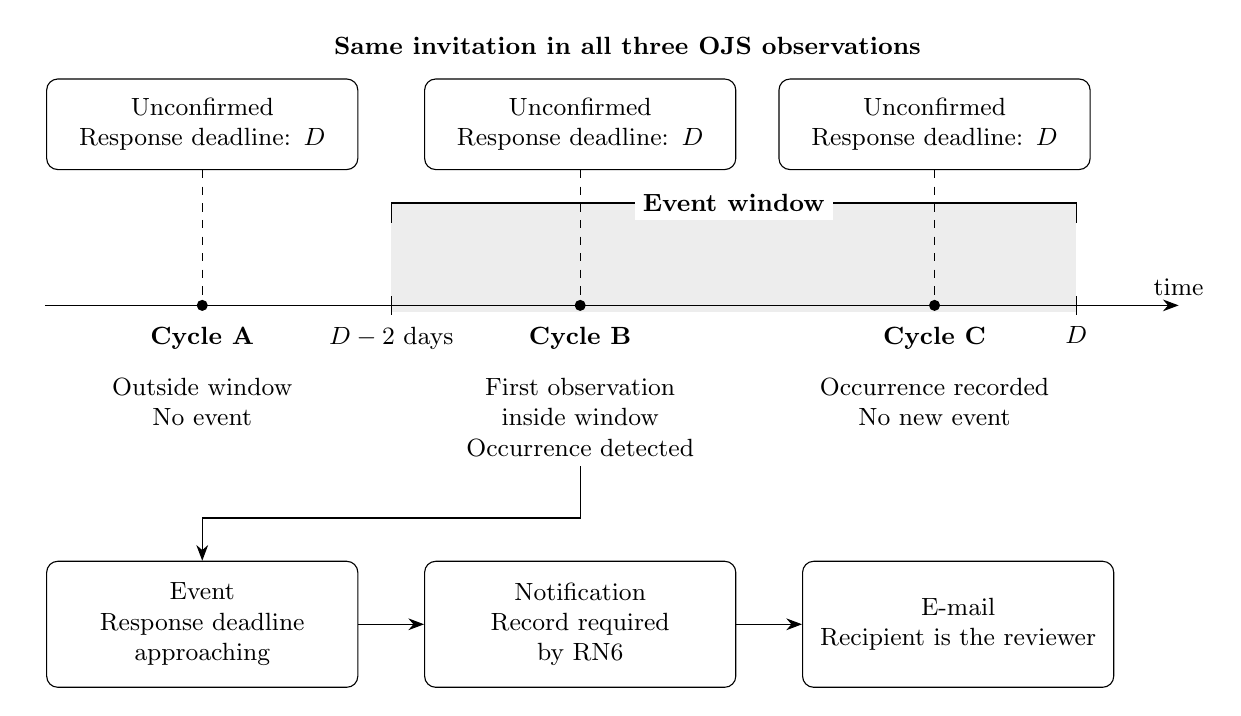
\begin{tikzpicture}[
  box/.style={draw,rounded corners,align=center,font=\small,
    text width=3.6cm,minimum height=1.15cm,inner sep=5pt},
  arr/.style={-{Stealth[length=2mm]}},
  note/.style={align=center,font=\small,text width=4.2cm,anchor=north}]
  \fill[black!7] (4,-.08) rectangle (12.7,1.3);
  \draw (4,1.05) -- (4,1.3) -- (12.7,1.3) -- (12.7,1.05);
  \node[font=\small\bfseries,fill=white,inner sep=3pt] at (8.35,1.3)
    {Event window};
  \node[font=\small\bfseries] at (7,3.3)
    {Same invitation in all three OJS observations};

  \node[box] (a) at (1.6,2.3) {Unconfirmed\\Response deadline: $D$};
  \node[box] (b) at (6.4,2.3) {Unconfirmed\\Response deadline: $D$};
  \node[box] (c) at (10.9,2.3) {Unconfirmed\\Response deadline: $D$};
  \draw[dashed] (a.south) -- (1.6,0);
  \draw[dashed] (b.south) -- (6.4,0);
  \draw[dashed] (c.south) -- (10.9,0);

  \draw[arr] (-.4,0) -- (14,0) node[above,font=\small] {time};
  \draw (4,-.12) -- (4,.12);
  \draw (12.7,-.12) -- (12.7,.12);
  \node[below,font=\small] at (4,-.15) {$D - 2$ days};
  \node[below,font=\small] at (12.7,-.15) {$D$};
  \foreach \x/\label in {1.6/A,6.4/B,10.9/C} {
    \fill (\x,0) circle (2pt);
    \node[below,font=\small\bfseries] at (\x,-.15) {Cycle \label};
  }

  \node[note] at (1.6,-.8) {Outside window\\No event};
  \node[note] (first) at (6.4,-.8) {First observation\\inside window\\Occurrence detected};
  \node[note] at (10.9,-.8) {Occurrence recorded\\No new event};

  \node[box,minimum height=1.6cm] (event) at (1.6,-4.05) {Event\\Response deadline\\approaching};
  \node[box,minimum height=1.6cm] (notice) at (6.4,-4.05) {Notification\\Record required\\by RN6};
  \node[box,minimum height=1.6cm] (request) at (11.2,-4.05) {E-mail\\Recipient is the reviewer};
  \draw[arr] (first.south) -- (6.4,-2.7) -| (event.north);
  \draw[arr] (event) -- (notice);
  \draw[arr] (notice) -- (request);
\end{tikzpicture}%
}
\endgroup
\caption{Time-based event detection (RN6). Source: the authors.}
\label{fig:notificacao-rn6}
\end{figure}

A \emph{finding} states that a submission needs the chief editor's
attention. It can stay open across several collection cycles without a
new event in each cycle. A missing editor is an example of such a
condition. A \emph{notification} is a record that a rule specifies, and it
produces one \emph{e-mail} per recipient. \emph{Curation} comprises the
human actions in the dashboard: notes, conference associations, muting,
and marks as up to date.

The monitoring requirements cover notices to editors about invitation
responses, missed deadlines, received reviews, completion of all reviews,
and signs of a revised manuscript. Reviewers receive notifications in
the two-day window before response and review deadlines, and an overdue
review notice. Chief editors can consult current findings in the
dashboard and in the editorial summary e-mail.

\subsection{Rules}

Table~\ref{tab:regras} lists the monitoring rules and their outputs.
At the
chief editors' request, the system requires two active reviewers per round.
It also waits seven days after a revision-request decision before RN11 and
RN16 apply. These are configurable journal-specific criteria.
Active reviewers are the assignments of the latest round in
the assignment that are not declined, cancelled, or overdue for a response.

\begin{table}[!t]
\caption{Monitoring rules and outputs. RN stands for business rule
(Portuguese: \textit{regra de negócio}). AE: assigned editor.}
\label{tab:regras}
\centering
\footnotesize
\begin{tabularx}{\textwidth}{@{}p{.8cm}X>{\raggedright\arraybackslash}p{4.3cm}@{}}
\toprule
Rule & Condition & Output \\
\midrule
RN1 & A reviewer answers an invitation (Section~\ref{sec:discussao}). & Invitation-answered notice to the AE. \\
RN2 & Invitation unanswered after its response due date. & Notice to the AE. \\
RN3 & Reviewer submits a review. & Notice to the AE. \\
RN4 & All reviews in the round become complete. & Notice to the AE. \\
RN5 & The latest round leaves the revisions-requested or resubmit-for-review state. & Revision-hint notice to the AE. \\
RN6 & Unanswered invitation in the 48 hours before its response due date. & Approaching-deadline notice to the reviewer. \\
RN7 & Incomplete review assignment in the two calendar days before its review due date. & Approaching-deadline notice to the reviewer. \\
RN8 & Incomplete review assignment from the start of its review due date. & Overdue notice to the reviewer. \\
RN9 & Latest open round with fewer than two active reviewers. & Missing-reviewer finding. \\
RN10 & Confirmed, incomplete review from the start of its review due date. & Overdue-review finding. \\
RN11 & Revision still pending more than seven days after the revision-request decision, with no later round. & Missing-revised-manuscript finding. \\
RN13 & Submission has no assigned editor. & Missing-editor finding. \\
RN15 & All reviews of the latest round are complete, with no later decision. & Reviews-complete-without-decision finding. \\
RN16 & Revision no longer pending, more than seven days after the revision-request decision, with no later round. & Revised-manuscript-awaiting-decision finding. \\
RN17 & Submission in the OJS \textit{Submission} stage, before a decision to send it to review. & Desk-decision finding. \\
RN18 & Observed absence of a \textit{Copyeditor} on an active submission in \textit{Copyediting}. & Finding, and a first notice to the assigned \textit{Journal editors}. \\
RN19 & Overdue invitation in the latest round, with fewer than two active reviewers. & Overdue-invitation finding. \\
\bottomrule
\end{tabularx}
\end{table}

\section{Development and Implemented Solution}
\label{sec:solucao}

For each rule, queries to OJS established which report, API resource, or
page provides the data. Development proceeded incrementally through data
collection, processing, messaging, and the interface.

\subsection{Architecture and Cycle Execution}

The Go server \cite{golang} extends PocketBase, which provides
authentication, an API, and SQLite persistence \cite{pocketbase,sqlite}.
It serves the Next.js dashboard as static files \cite{nextestatico} behind
a Caddy reverse proxy \cite{caddy}. Figure~\ref{fig:arquitetura}
shows the components and the data exchanges. The SMTP server is an
external dependency.

\begin{figure}[htbp]
\centering
\begingroup
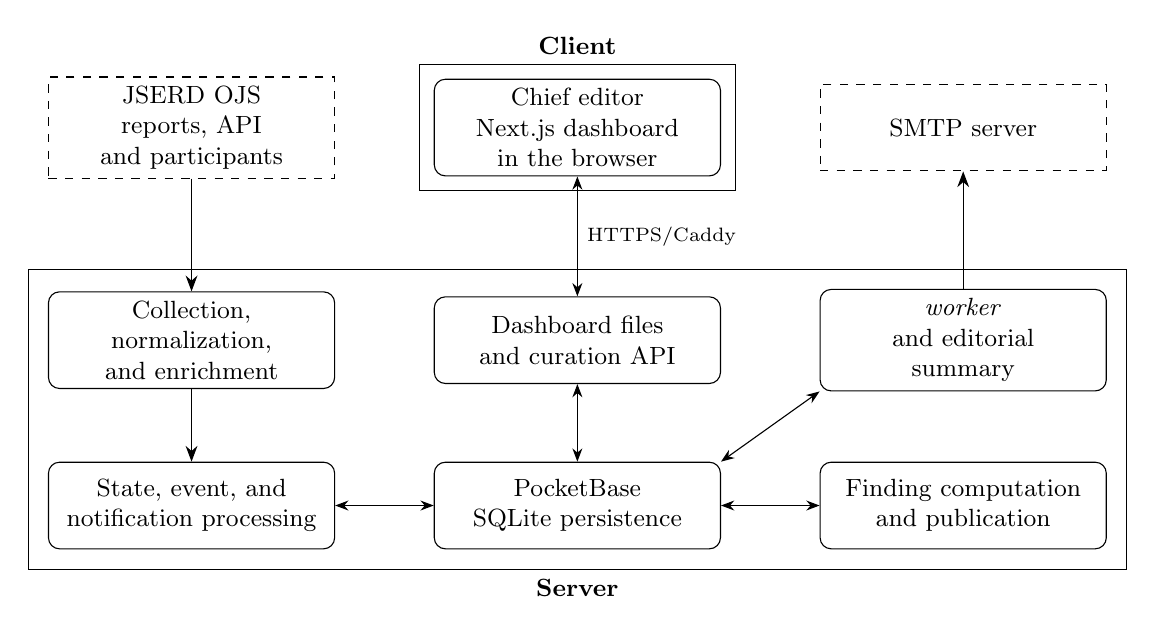
\begin{tikzpicture}[
  box/.style={draw,rounded corners,align=center,font=\small,text width=3.4cm,minimum height=1.1cm},
  ext/.style={draw,dashed,align=center,font=\small,text width=3.4cm,minimum height=1.1cm},
  arr/.style={-{Stealth[length=2mm]}}]
  \node[ext] (ojs) at (0,.6) {JSERD OJS\\reports, API\\and participants};
  \node[box] (web) at (4.9,.6) {Chief editor\\Next.js dashboard\\in the browser};
  \node[draw,fit=(web),inner sep=.18cm,
    label={[font=\small\bfseries]above:Client}] {};
  \node[ext] (smtp) at (9.8,.6) {SMTP server};
  \node[box] (collect) at (0,-2.1) {Collection,\\normalization,\\and enrichment};
  \node[box] (api) at (4.9,-2.1) {Dashboard files\\and curation API};
  \node[box] (mail) at (9.8,-2.1) {\textit{worker}\\and editorial\\summary};
  \node[box] (process) at (0,-4.2) {State, event, and\\notification processing};
  \node[box] (db) at (4.9,-4.2) {PocketBase\\SQLite persistence};
  \node[box] (find) at (9.8,-4.2) {Finding computation\\and publication};
  \node[draw,fit=(collect)(process)(find)(db)(mail)(api),inner sep=.25cm,
    label={[font=\small\bfseries]below:Server}] {};
  \draw[arr] (ojs) -- (collect);
  \draw[arr] (collect) -- (process);
  \draw[<->,>=Stealth] (process) -- (db);
  \draw[<->,>=Stealth] (find) -- (db);
  \draw[<->,>=Stealth] (db) -- (api);
  \draw[<->,>=Stealth] (db.north east) -- (mail.south west);
  \draw[arr] (mail) -- (smtp);
  \draw[<->,>=Stealth] (api) -- node[right,font=\scriptsize]{HTTPS/Caddy} (web);
\end{tikzpicture}
\endgroup
\caption{Architecture and data exchanges. Solid outlines enclose the client and server. Dashed boxes denote external dependencies. Source: the authors.}
\label{fig:arquitetura}
\end{figure}

A \emph{cycle} is the recurring unit of monitoring. By default, a cycle
runs every hour, the e-mail worker every minute, and the editorial summary
on Mondays at 09:00, São Paulo time. The superuser can also request a
manual cycle. The coordinator controls the cycle sequence and rejects a
second run while a cycle is in progress in the same process. The design
assumes one server process. Collection signs in, downloads the article and
review reports, and reads the submissions API. It records the source and
outcome of each download, including failures.

Normalization converts the data into a common internal model.
\emph{Enrichment} adds details from individual submission queries.
Processing stores the normalized state, compares it with the previous
state, detects events, and matches notification rules. The server then
computes findings, updates the dashboard, and checks the summary schedule.

Enrichment runs twice in each cycle. The first pass runs before the server
saves the snapshot, because RN2, RN5, RN7, RN8, and RN18 need live OJS
status to create events. The second pass runs before finding computation.
It reloads the saved snapshot and queries invitation status, due-date
status, and the active reviewers of the latest round again. A failed query stops the cycle. Committed transactions remain, and
the next cycle queries OJS again. If the second pass fails, the snapshot
and events remain, and the dashboard keeps its previous findings until the
next successful cycle.

\subsection{Combining Sources and Evidence}
\label{sec:fontes}

Collection reads three OJS sources. The \textit{ArticleReportPlugin},
\textit{ReviewReportPlugin}, and \textit{ViewReportPlugin} reports provide
submissions, assignments, and metrics in batches. The REST API lists
submissions with a summary schema, and an individual query returns stage,
rounds, and assignments \cite{pkpapi}. The stage participant page lists the
people assigned to each stage. The collection account needs access to all
three sources. The server queries details only for submissions that are
candidates for rules that need them.

The sources identify people differently. The Reviews report gives each
reviewer a username and an e-mail address, and reviewer notices go to that
address. The participant page gives only the names of assigned editors.
The system matches these names with the editor e-mail addresses in the
article report. The API detail gives the status and due date of each
assignment, but no reviewer identity. The system therefore applies API
status to all report rows that share a round, or a round and a review due
date.

For RN5, an author revision is pending when the latest round is in the
revisions-requested or resubmit-for-review state \cite{pkplib}. The event
occurs when a cycle observes the round in another state after the previous
cycle observed it as pending. The new state can be a submitted revision,
but also an accept or decline decision. RN5 is therefore an indicator that
can produce false positives, and it does not confirm a file or its author.
RN16 uses the same round-state proxy.

RN18 distinguishes an assigned \textit{Copyeditor}, an observed absence,
and unknown evidence. Only an observed absence produces a finding. Evidence
is unknown, for example, when the article report shows a submission in
\textit{Copyediting} but the individual query no longer does.

\subsection{Successive States and Duplicate Prevention}

The system stores a \emph{snapshot}, a copy of the normalized state, for
each processed cycle. Snapshot comparison detects transitions without
changes to OJS. The first snapshot is the baseline for transitions, but it
can already produce time-based and missing-copyeditor events.

Each event receives a key computed from its type, entity, transition, and
occurrence. For time-based events, the occurrence includes the deadline,
so a deadline extension produces a new event. The database enforces key
uniqueness, so reprocessing an occurrence creates no new record, as in the
\textit{Idempotent Receiver} pattern \cite{idemreceiver}.

One transaction records the cycle, the snapshot, and the events. A second
transaction creates the notification and one e-mail record per recipient
before any SMTP communication. Only this second step applies the
\textit{Transactional Outbox} pattern \cite{outbox}. Uniqueness constraints
and the worker reservation give three guarantees: at most one event per
key, one notification per event and rule, and one send attempt per e-mail.

\subsection{Notifications and Editorial Summary}

The e-mail worker reserves pending e-mails and records the outcome of each
send attempt. The persisted reservation prevents two workers from
processing the same e-mail. The first
notification to a person also produces a welcome e-mail.

Sending uses SMTP \cite{smtp} or the default simulated transport, which
writes e-mails to the server output. The templates are in English, have
plain-text and HTML versions, and are part of the code. A failure to create
a notification does not stop finding computation, and later cycles resume
event-rule matches without a notification.

\subsection{Dashboard and Preservation of Curation}

The dashboard lists submissions with their findings and the supporting
data. The work list orders submissions by their most severe finding.
The detail view shows OJS evidence, send history, and curation notes,
with a link to the submission in OJS. The dashboard is available in
Portuguese and English. Figure~\ref{fig:painel} shows the work list and the
send history of one submission with fictitious data.

\begin{figure}[!t]
\centering
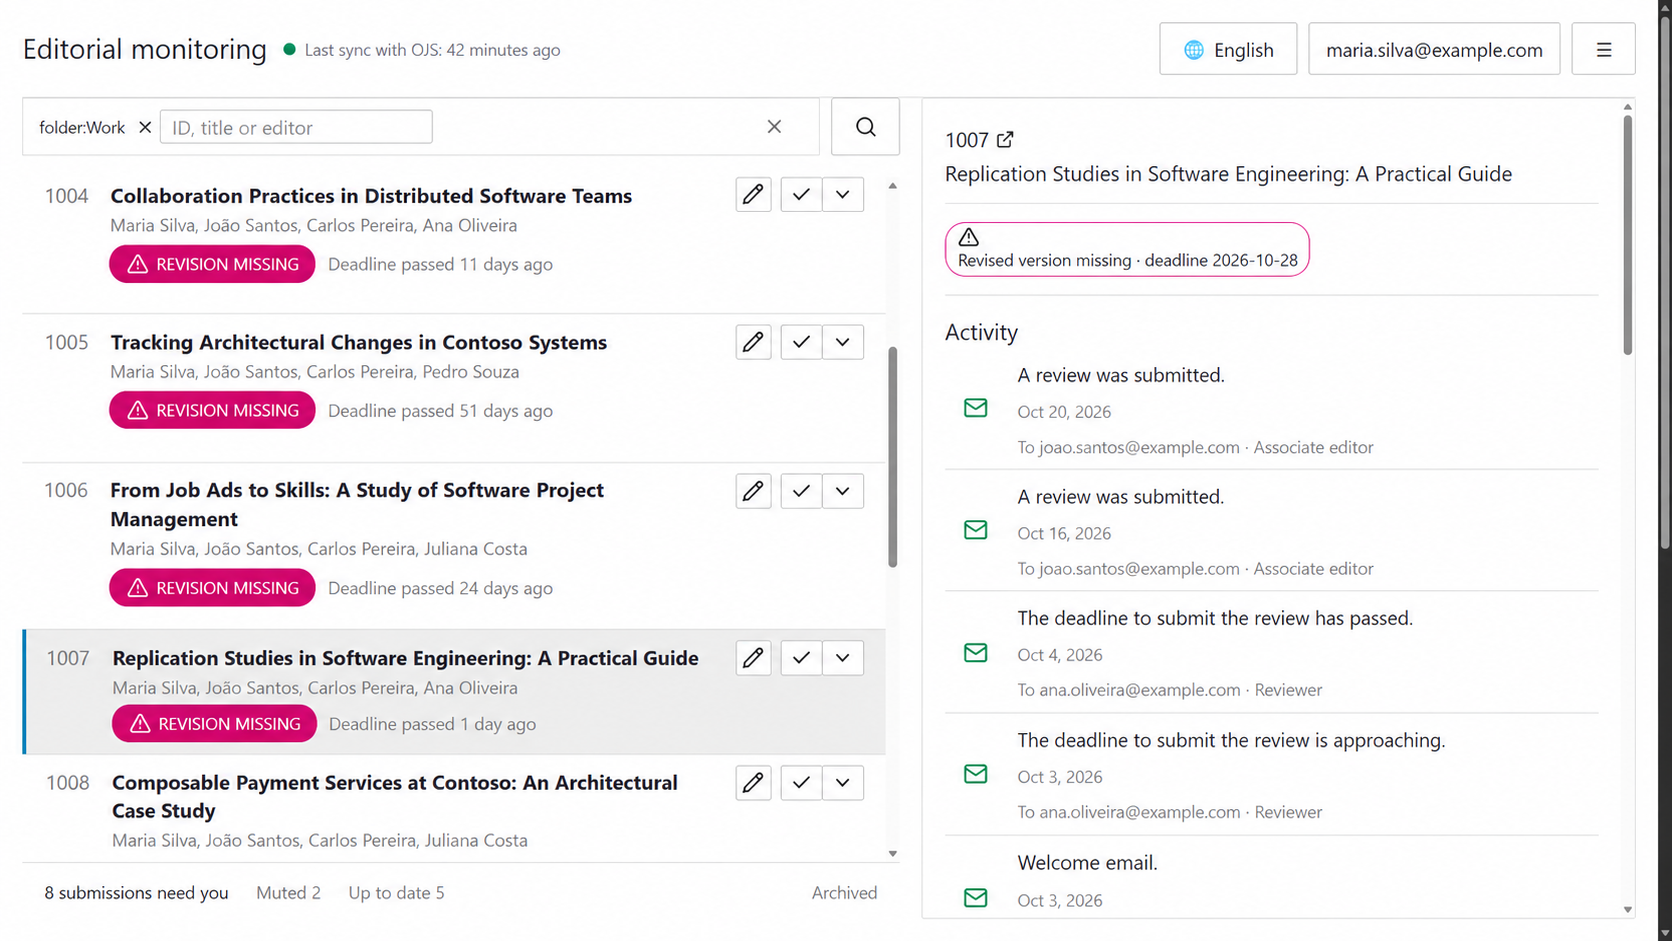
\includegraphics[width=\linewidth]{painel-monitoramento-editorial.png}
\caption{Dashboard with the work list and a selected submission. All data are fictitious. Source: the authors.}
\label{fig:painel}
\end{figure}

Each submission belongs to exactly one queue, assigned in this order:
archived, muted, up to date, and work (Figure~\ref{fig:filas}). Final
outcomes, such as publication, rejection, and withdrawal, depend on the
current OJS state.

\begin{figure}[!t]
\centering
\begingroup
\resizebox{\linewidth}{!}{%
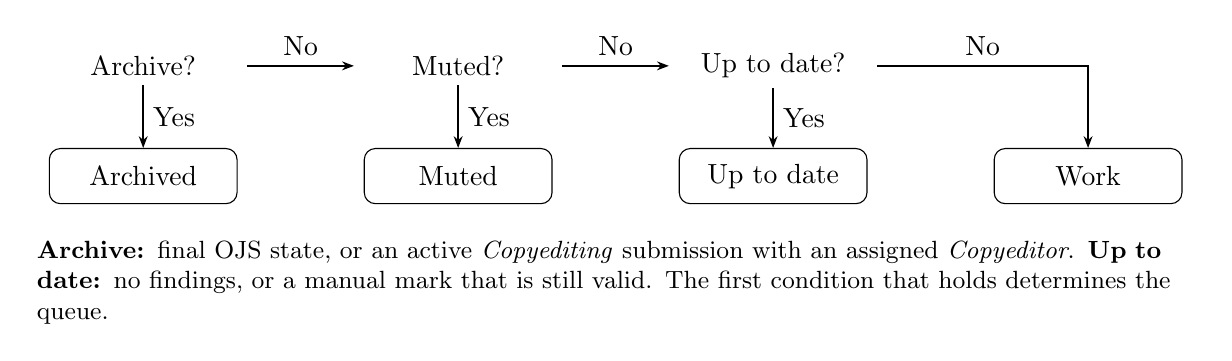
\begin{tikzpicture}[
 font=\fontsize{10}{12}\selectfont,
 arr/.style={-{Stealth[length=1.5mm]},semithick},
 queue/.style={draw,rounded corners,align=center,text width=2.15cm,minimum height=.7cm},
 note/.style={align=left,text width=14.7cm,font=\fontsize{9}{11}\selectfont,anchor=north}]

\node[align=center,text width=2.4cm] (a) at (0,0) {Archive?};
\node[align=center,text width=2.4cm] (b) at (4,0) {Muted?};
\node[align=center,text width=2.4cm] (c) at (8,0) {Up to date?};
\node[queue] (ar) at (0,-1.4) {Archived};
\node[queue] (mu) at (4,-1.4) {Muted};
\node[queue] (up) at (8,-1.4) {Up to date};
\node[queue] (wo) at (12,-1.4) {Work};
\draw[arr] (a) -- node[above]{No} (b);
\draw[arr] (b) -- node[above]{No} (c);
\draw[arr] (c.east) -- node[above]{No} (12,0) -- (wo.north);
\draw[arr] (a) -- node[right]{Yes} (ar);
\draw[arr] (b) -- node[right]{Yes} (mu);
\draw[arr] (c) -- node[right]{Yes} (up);
\node[note] at (6,-2.1) {\textbf{Archive:} final OJS state, or an active \textit{Copyediting} submission with an assigned \textit{Copyeditor}. \textbf{Up to date:} no findings, or a manual mark that is still valid. The first condition that holds determines the queue.};

\end{tikzpicture}%
}
\endgroup
\caption{Dashboard queue precedence. Arrows show the classification order. Source: the authors.}
\label{fig:filas}
\end{figure}

When a chief editor marks a submission as up to date, the system saves a
digest of the finding types present at that moment, without deadlines or
counts. The mark expires when the set of types changes or when the return
date that the chief editor chose arrives.

Muting removes a submission from the work list when a trusted editor
handles it. Conference associations exist only in JSERD Monitoring. A
trusted editor handles the submissions of a conference, so selecting or
changing a conference also mutes the submission, and removing the
association unmutes it. The chief editor can still unmute a submission and
keep its conference. The system still collects and evaluates muted
submissions, but their findings do not return them to the work list. Muting
also removes a submission from the editorial summary, but editors and
reviewers still receive event notifications.

Curation data remain separate from data that the system recomputes. A new
cycle can update the state and findings of a submission, but notes are
immutable. Access follows the same split. Chief editors change curation
data, and only the superuser administers the server.

\subsection{Access, Personal Data, and Availability}

The dashboard requires chief editor authentication and shows the same
journal view to every account. The OJS and SMTP credentials reach the server as
environment variables from a file on the host.

The database contains submission and assignment data, contact data for
authors, editors, and reviewers, and curation records. Following the necessity principle in
Art.~6 of the LGPD \cite{lgpd}, snapshots do not keep review comments,
recommendations, or reviewer profile columns, which no rule reads. The raw
report files keep every column, including review comments. Retention keeps
raw files and snapshot contents for the 240 most recent cycles, about ten
days at the default schedule. A daily off-site backup contains the
PocketBase databases and the latest state, but not the full history of raw
files and states.

\section{Related Work}
\label{sec:relacionados}

Journal systems offer part of this monitoring. OJS 3.2 sends reviewer
reminders after due dates \cite{pkpworkflow}, and it e-mails stage editors
when a reviewer accepts or declines an invitation \cite{pkplib}.
JSERD Monitoring adds rules that
combine several sources, findings for chief editors, and local curation,
without changes to OJS.

Lopes and Oliveira describe a framework that queries sources periodically,
compares the results with internal storage, and triggers template-defined
operations, including e-mails, for unrecorded content \cite{lopes2015}. It
detects new content through identifiers or hashes. JSERD Monitoring
compares normalized states to detect editorial transitions, and other rules
consider elapsed time and persistent conditions.

Labio and Garcia-Molina \cite{labio1996} study snapshot comparison to infer
changes. Duplicate prevention relates to the \textit{Idempotent Receiver}
pattern \cite{idemreceiver}, and the e-mail records relate to the
\textit{Transactional Outbox} pattern \cite{outbox}.

\section{Discussion and Limitations}
\label{sec:discussao}

The article report and the participant page identify editors by name,
without a stable identifier. Name normalization merges people with the
same name, also across the editor and reviewer roles. The API detail has
no reviewer identity. The Reviews report keeps declined and cancelled
assignments, and a decline also fills the confirmation date
\cite{pkplib}.

Periodic collection delays change detection. A cycle represents the data
that its queries obtained. Report and detail queries do not form a single
OJS transaction. Transitions before observation began have no previous
state, and intermediate changes between cycles can go unobserved.

The integration depends on permissions, report plugins, the structure of
participant pages, and OJS status codes \cite{pkplib}, and not all of them
have a stable interface. Another OJS version or journal requires a check of
these sources and of local criteria.

A prepared notification does not guarantee delivery. Missing addresses
prevent sending. The worker does not retry failed attempts. Ordering
is not guaranteed, and SMTP acceptance does not prove arrival or reading.
The design therefore does not give the delivery guarantees of the
\textit{Transactional Outbox} pattern.

\section{Conclusion}
\label{sec:conclusao}

JSERD Monitoring is an external monitoring layer for the OJS installation
of JSERD, while editorial decisions remain in OJS. The server combines
reports and individual queries, stores successive states, recognizes events,
computes findings, and prepares notifications.
The implementation combines sources according to the data each rule
requires, separates events from persistent conditions, and preserves
human records between collection cycles. Adapting it to another journal
requires reviewing local criteria, permissions, and OJS interface
contracts.

\bibliographystyle{sbc}
\bibliography{sbc-jheam-ross}
\end{document}
